\documentclass[runningheads]{llncs}
%
\usepackage[T1]{fontenc}
% T1 fonts will be used to generate the final print and online PDFs,
% so please use T1 fonts in your manuscript whenever possible.
% Other font encondings may result in incorrect characters.
%
\usepackage{graphicx}
% Used for displaying a sample figure. If possible, figure files should
% be included in EPS format.
%
% If you use the hyperref package, please uncomment the following two lines
% to display URLs in blue roman font according to Springer's eBook style:
%\usepackage{color}
%\renewcommand\UrlFont{\color{blue}\rmfamily}
%
\begin{document}
%
\title{Formalization and Runtime Verification of Invariants for
Robotic Systems}
%
%\titlerunning{Abbreviated paper title}
% If the paper title is too long for the running head, you can set
% an abbreviated paper title here
%
\author{Ricardo Cordeiro\inst{1} \and
Alcides Fonseca\inst{1} \and
Christopher S. Timperley\inst{2}}
%\orcidID{0000-0002-8959-1702}
%
\authorrunning{Ricardo Cordeiro et al.}
% First names are abbreviated in the running head.
% If there are more than two authors, 'et al.' is used.
%
\institute{Faculdade de Ciências da Universidade de Lisboa,
Lisboa, Portugal \and
Carnegie Mellon University, Pittsburgh, PA}
%
\maketitle              % typeset the header of the contribution
%
\begin{abstract}
    Robotic systems are critical in today's society, a potential failure in a robot may have extraordinary costs, not only financial, but can also cost lives.
    Current practices in robot testing are vast and involve methods like simulation, log checking, or field testing. However current practices often require human visualization to determine the correctness of a given behavior. Automating this analysis can not only relieve the burden from a high-skilled engineer, but also allow for massive parallel executions of tests, that can detect behavioral faults in the robots that would otherwise not be found due to human error or lack of time.
    We have developed a DSL (domain-specific language) to specify properties of robotic systems in ROS. Specifications written by developers in this language are compiled to a monitor ROS (Robot Operating System) module, that detects violations of those properties in runtime. We have used this language to express the temporal and positional properties of robots, and we have automated the monitoring of some behavioral violations of robots in relation to their state or events during a simulation.

\keywords{Robotics  \and Domain-specific language \and Runtime Monitoring \and Error detection.}
\end{abstract}
%
%
%
\section{Introduction}

Robotics already have a great impact on our current society. Due to their broad practicality, the quality of software used by robots should be of extreme importance to us. Robotic Systems are non-deterministic, mainly because robots interact directly with the real world. A sensor can return imprecise values since the environment itself can be very hard to predict. As a result, verifying whether a task or movement is correct can be difficult for a system to conceive.

ROS is an open-source framework with a vast collection of libraries, interfaces, and tools that help build robot software. ROS provides an abstraction between hardware and software that helps developers easily connect the different robot components through what are called "topics" and "messages".

Current practices in testing robot software mainly involve field testing, simulation testing, and log checking and require a human to analyze the behavior of the robot to determine whether the behavior is correct.

The objective of this work~\cite{github_repo} is to show how a domain-specific language can be used to specify temporal and positional properties of robotic systems and monitor the simulation components associated with these properties.

The language allows describing a robotic system's properties in a somewhat simple and intuitive way, while at the same time still being able to express relevant temporal and positional arguments between robots and objects in the simulation. The language is supported by a compiler. The compiler translates the language to a monitoring mechanism. In this way, if a robotic system doesn't follow the properties defined by the user writing in the language, during execution, the compiler detects an anomaly and makes the analysis that the behavior of the robot is not consistent. This is possible because in simulation the developers can take advantage of real values of objects' attributes to compare with what the robot system perceives.

*Mention related work?*

The paper starts with a motivational example of a hypothetical scenario, followed by an overall explanation of the approach, afterward is presented the language in more detail, and finally, a conclusion on the work is presented.

\section{Motivational Example}

If a developer of an autonomous moving car wanted to express that the robot always needs to stop when going near a stop sign, he could write something like:

\vspace{3mm}

\texttt{after\_until robot.distance.stop\_sign < 1, robot.distance.stop\_sign > 1, eventually robot.velocity == 0}

\vspace{3mm}

Translating to a more human language we are saying that, after the robot's distance to the stop-sign is below the value of 1 in the simulator, up until the distance is again above 1, the robot velocity will eventually be equal to 0.

The specified property is compiled and a python file is generated which is capable of running as a ROS node. The node listens to relevant topics and performs the computations to verify the specified property.

\begin{figure}
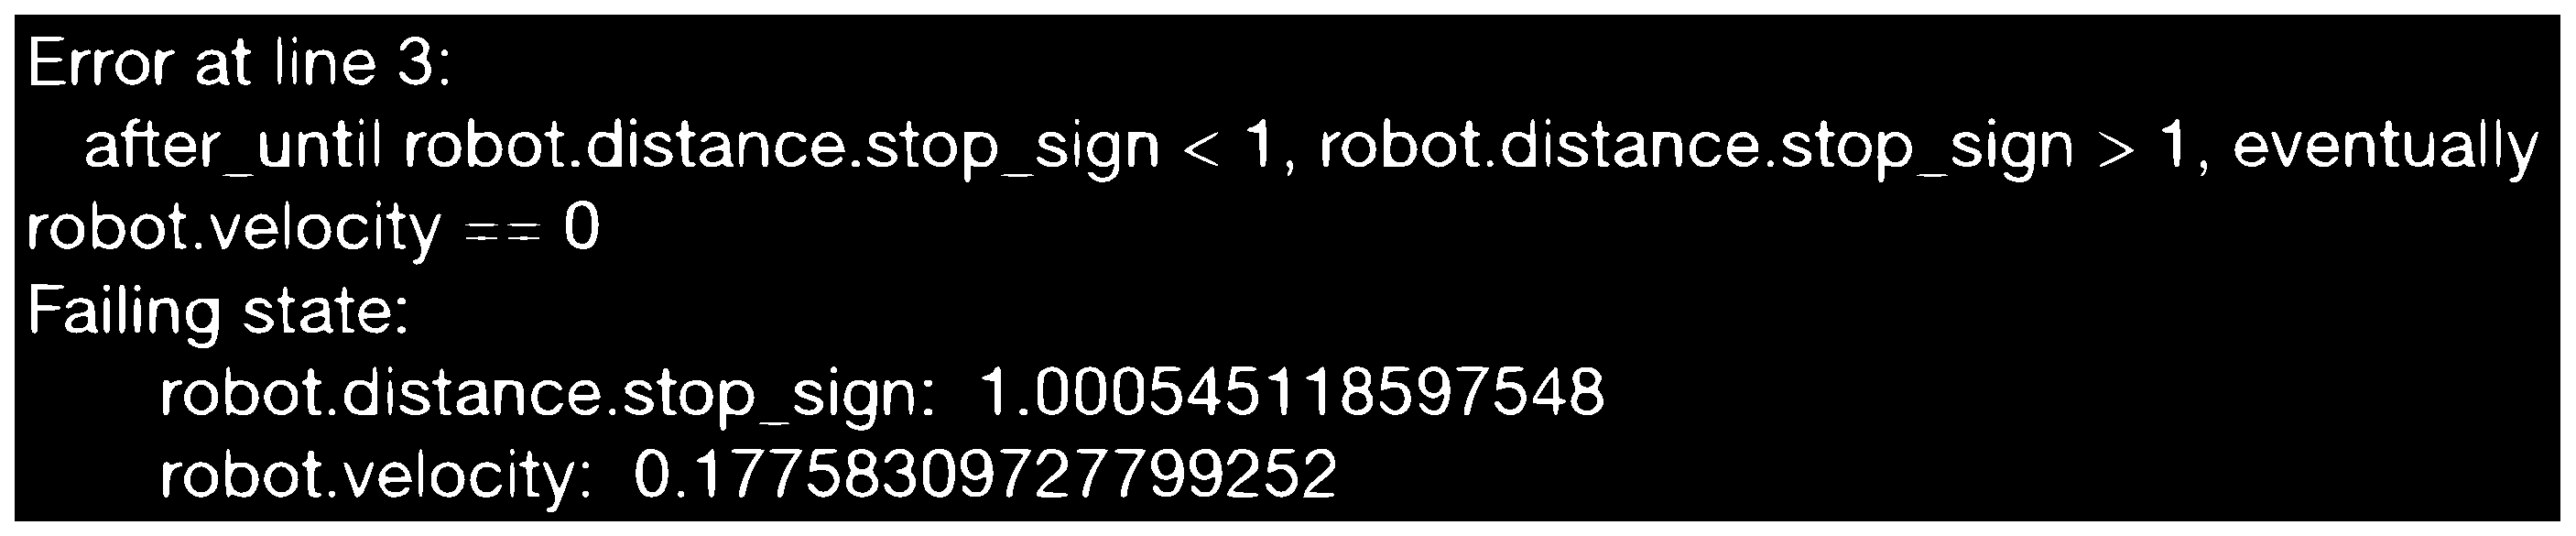
\includegraphics[width=\textwidth]{error.eps}
\caption{Example of the displayed error when the robot doesn't stop at the stop sign.} \label{fig1}
\end{figure}

\section{Approach}

\begin{figure}
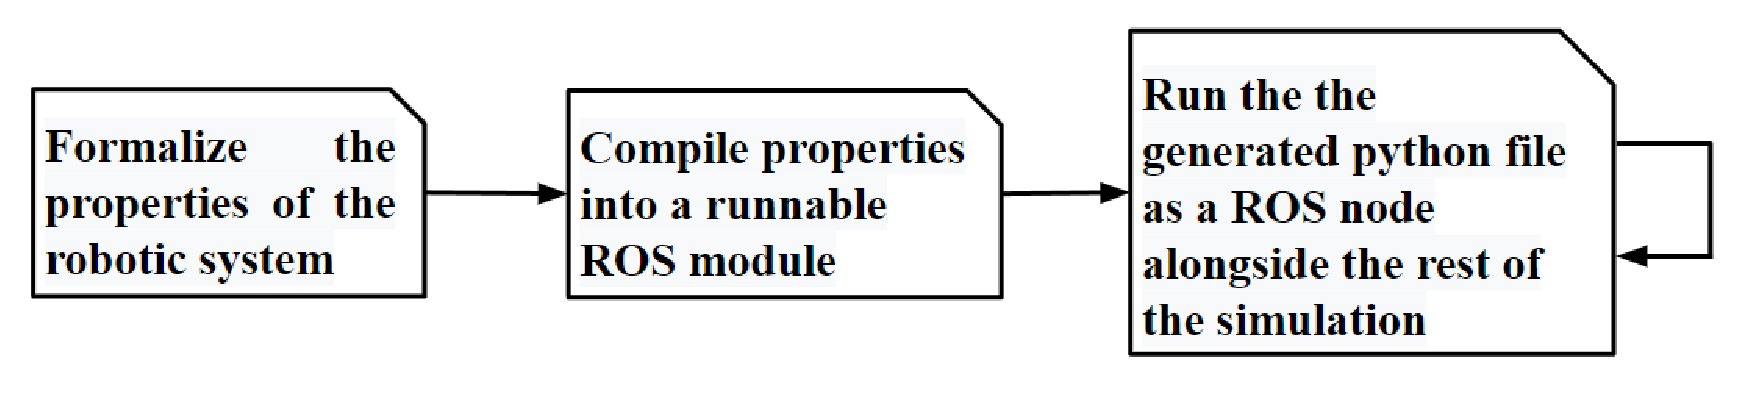
\includegraphics[width=\textwidth]{diagram.eps}
\caption{Flow of the process for runtime verification.} \label{fig2}
\end{figure}

The diagram in Fig.2 represents the flow of the process of monitoring a robotic system. 

First, there is a need of writing in the DSL the properties of the robotic system one wants to monitor in a .txt file extension.

Afterward, the specified properties need to be compiled and a python file is generated which is capable of running as a ROS node.

Finally, the node can be run whenever testing the system and will listen to relevant topics and perform the computations needed to verify the specified properties.


\section{Language Features}

The domain-specific language relies on an adaptation of linear temporal logic to express temporal relations of and between simulation objects.

The domain-specific language also has shortcuts to express the absolute values of certain useful concepts of objects in a simulation.

\subsection{Temporal Keywords}

\begin{itemize}
\item {\bfseries always X} - X has to hold on the entire subsequent path;
\item {\bfseries never X} - X never holds on the entire subsequent path;
\item {\bfseries eventually X} - X eventually has to hold, somewhere on the subsequent path;
\item {\bfseries after X, Y} - after the event X is observed, Y has to hold on the entire subsequent path;
\item {\bfseries until X, Y} - X holds at the current or future position, and Y has to hold until that position. At that position, Y does not have to hold anymore;
\item {\bfseries after\_until X, Y, Z} - after the event X is observed, Z has to hold on the entire subsequent path up until Y happens, at that position Z does not have to hold anymore;
\end{itemize}

\noindent It is also possible to reference previous variable states:
\begin{equation}
    @\{X, -y\}
\end{equation}
This will represent the value of the variable X in the point in time -y.

\subsection{Useful Predicates}

\begin{itemize}
\item {\bfseries X.position} - The position of the robot in the simulation;
\item {\bfseries X.position.y} - The position in the y axis of the robot in the simulation. Also works for x and z;
\item {\bfseries X.distance.Y} - The absolute distance between two objects in the simulation. For the x and y axis;
\item {\bfseries X.distanceZ.Y} - The absolute distance between two objects in the simulation. For the x, y, and z axis;
\item {\bfseries X.velocity} - The velocity of an object in the simulation. This refers to linear velocity;
\item {\bfseries X.velocity.x} - The velocity in the x axis of an object in the simulation. This refers to linear velocity;
\item {\bfseries X.localization\_error} - The difference between the robot's perception of its position and the actual position in the simulation;
\end{itemize}

\subsection{Examples}

As an example, we specify two properties for an arbitrary robotic system of autonomous driving robots:

\subsubsection{Property One}:

The robot velocity will never be above 2 for the duration of the simulation;

\vspace{3mm}

\texttt{never robot.velocity > 2.0}

\subsubsection{Property Two}:

The first robot being above 1 velocity implies that the second robot is at least at 0.8 distance from the first robot. Up until they reach a certain location;

\vspace{3mm}

\texttt{until (robot1.position.x > 45 and robot1.position.y > 45), always (robot1.velocity > 1 implies robot2.distance.robot1 > 0.8)}


\section{Conclusion}

Robotics and ROS usage in specific has been constantly growing. With more robot software the need for and the probability of errors not found by human-in-the-loop testing will also grow.

With the proposed approach we hope to illustrate how a DSL can potentially help automate the monitoring of unwanted behaviors in robotic systems.


\begin{thebibliography}{8}
%\bibitem{ref_article1}
%Author, F.: Article title. Journal \textbf{2}(5), 99--110 (2016)

%\bibitem{ref_lncs1}
%Author, F., Author, S.: Title of a proceedings paper. In: Editor,
%F., Editor, S. (eds.) CONFERENCE 2016, LNCS, vol. 9999, pp. 1--13.
%Springer, Heidelberg (2016). \doi{10.10007/1234567890}

%\bibitem{ref_book1}
%Author, F., Author, S., Author, T.: Book title. 2nd edn. Publisher,
%Location (1999)

%\bibitem{ref_proc1}
%Author, A.-B.: Contribution title. In: 9th International Proceedings
%on Proceedings, pp. 1--2. Publisher, Location (2010)

\bibitem{github_repo}
GitHub repository of the work, \url{https://ricardocajo.github.io/error-monitor-ros-gazebo}
\end{thebibliography}
\end{document}
